\section{Dimensionality Reduction using PCA}
For the following data points, find the first principal component and then project the data
points onto it.
\begin{figure}[H]
    \centering
    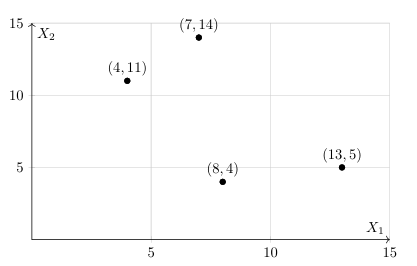
\includegraphics[width=0.7\textwidth]{chart1.png}
\end{figure}
\begin{qsolve}
    \begin{qsolve}[]
        first we define $X$ as the matrix of data points:
        $$X = \begin{bmatrix}
            4 & 11\\
            7 & 14\\
            8 & 4\\
            13 & 5
            \end{bmatrix}$$
        we can define the covariance matrix as:
        $$S = \frac{1}{n}(X^TX- \frac{1}{n}X^T1_n1_n^TX)$$
        where $1_n$ is a vector of ones of size $n$.\\
        \splitqsolve[\splitqsolve]
        so we have:
        $$S = \frac{1}{4}\begin{bmatrix}
            4 & 7 & 8 & 13\\
            11 & 14 & 4 & 5
            \end{bmatrix}\begin{bmatrix}
            4 & 11\\
            7 & 14\\
            8 & 4\\
            13 & 5
            \end{bmatrix} - \frac{1}{4}\begin{bmatrix}
            4 & 7 & 8 & 13\\
            11 & 14 & 4 & 5
            \end{bmatrix}\begin{bmatrix}
            1 & 1 & 1 & 1\\
            1 & 1 & 1 & 1\\
            1 & 1 & 1 & 1\\
            1 & 1 & 1 & 1
            \end{bmatrix}\begin{bmatrix}
            4 & 11\\
            7 & 14\\
            8 & 4\\
            13 & 5
            \end{bmatrix}$$
        so we have:
        $$S = \begin{bmatrix}
            10.5 & -8.25\\
            -8.25 & 17.25
        \end{bmatrix}$$
        now we can find the eigenvalues and eigenvectors of $S$:
        $$det(S-\lambda I) = 0$$
        $$det\begin{bmatrix}
            10.5-\lambda & -8.25\\
            -8.25 & 17.25-\lambda
        \end{bmatrix} = 0$$
        $$\Rightarrow \lambda_1 = 22.79, \lambda_2 = 4.68$$
        $$\Rightarrow v_1 = \begin{bmatrix}
            0.5574\\ 
            -0.8303
        \end{bmatrix}, v_2 = \begin{bmatrix}
            0.8303\\ 
            0.5574
        \end{bmatrix}$$
        so the first principal component is $v_1$ and the projection of the data points onto it is:
        $$Xv_1 = \begin{bmatrix}
            4 & 11\\
            7 & 14\\
            8 & 4\\
            13 & 5
            \end{bmatrix}\begin{bmatrix}
            0.5574\\ 
            -0.8303
        \end{bmatrix} = \begin{bmatrix}
            -6.9037\\
            -7.7224\\
            1.138\\
            3.0947
        \end{bmatrix}$$
    \end{qsolve}
\end{qsolve}